\section{ХОД РАБОТЫ}

% choice
\subsection{Выбор метода пронозирования для каждого из товаров}

Существуют некоторые рекомендации по выбору метода прогнозирования в 
зависимости от исходных значений спроса за прошедший период.

Если величина, для которой требуется найти прогноз, имеет достаточно
чёткую тенденцию к росту или, наоборот, к снижению, то для такой величины
подходящей обычно оказывается регрессионная модель. При отсутствии такой
тенденции (то есть если исследуемая величина в некоторые периоды росла,
а в некоторые --- снижалась) более подходящими могут оказаться методы
скользящего среднего или экспоненциального сглаживания.

Построим график зависимости значения фактического спроса за период
для каждого из товаров. Из рисунка~\ref{fig:initial} видно, что
фактический спрос второго товара имеет чёткую тенденцию к снижению.
Таким образом, для прогнозирования будет использован метод линейной регрессии.

\begin{figure}[h!]
  \centering
  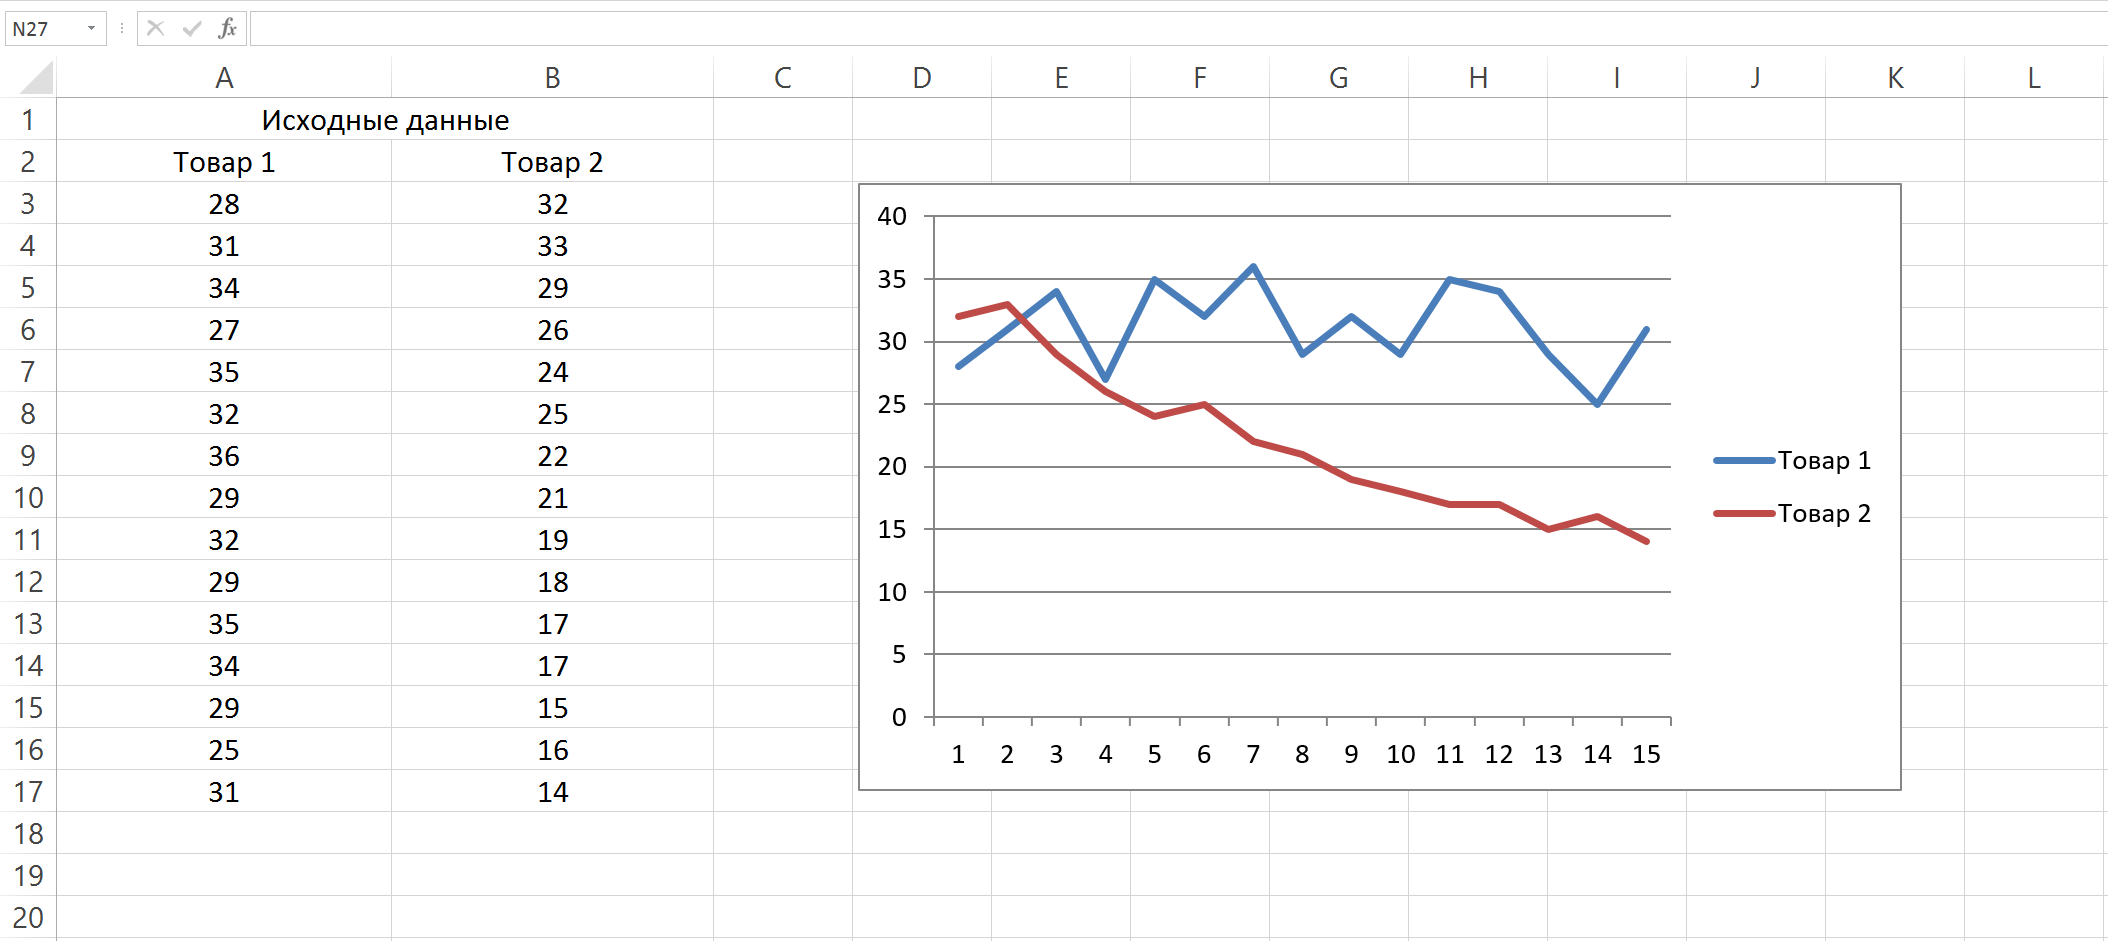
\includegraphics[width=150mm]{pic/initial}
  \caption{Исходные данные}
  \label{fig:initial}
\end{figure}

Значения фактического спроса на первый товар не имеют чёткой тенденции.
Значит для прогнозирования фактического спроса на этот товор следует
использовать метод скользящего среднего или экспоненциального сглаживания.


\subsection{Товар 1. Прогноз методом скользящего среднего}

% theory
Суть метода скользящего среднего: пусть имеются значения некоторой
величины за $n$ периодов $y_1, y_2, \dots, y_n$.
Прогноз величины $\hat{y}_{n+1}$ на $(n+1)\text{-ый}$ период определяется как
среднее значение за $k$ последних периодов.

Используя этот метод с периодом $k=2$ найдём прогноз на 16-ый период
для первого товара. Для этого воспользуемся инструментом
<<Скользящее среднее>> MS Excel c параметрами:
\begin{itemize}
  \item входной интервал --- ячейки с фактическими данными;
  \item интервал --- 2;
  \item выходной интервал --- ячейка, с которой начнется вывод результата~(со смещением).
\end{itemize}


% k = 2
Рассмотрим, например, как вычислен прогноз на 3-й и 4-й период. Также найдём
прогноз спроса на 16-й период.
\begin{align*}
  \hat{y}_3 &= \dfrac{y_1 + y_2}{2} = \dfrac{28 + 31}{2} = 29{,}5, \\
  \hat{y}_4 &= \dfrac{y_2 + y_3}{2} = \dfrac{31 + 34}{2} = 32{,}5, \\
  \hat{y}_{16} &= \dfrac{y_{14} + y_{15}}{2} = \dfrac{25 + 31}{2} = 28{,}0.
\end{align*}

Для оценки точности этого алгоритма найдём среднее абсолютное отклонение
(\textit{Mean Absolute Deviation, MAD}) фактических данных от прогнозируемых по формуле:
\[
  MAD_{k=2} = \dfrac{\sum_{i=1}^{m} |\hat{y}_i - y_i| }{m} = \dfrac{|\hat{y}_3 - y_3| + |\hat{y}_4 - y_4| + \dots + |\hat{y}_{15} - y_{15}|}{13} = 3{,}65.
\]

Повторно воспользуемся методом скользящего среднего с периодом $k=3$.
Стоит отметить, что прогноз на определённый период в данном случае строится
по трём предыдущим значениям, поэтому первая прогнозируемая величина будет
прогнозом спроса на товар за четвёртый период.

% k = 3
Вычисление прогноза на 3-й, 4-й и 16-й период соответственно:
\begin{align*}
  \hat{y}_4 &= \dfrac{y_1 + y_2 + y_3}{3} = \dfrac{28 + 31 + 34}{3} = 31{,}0, \\
  \hat{y}_5 &= \dfrac{y_2 + y_3 + y_4}{3} = \dfrac{31 + 34 + 27}{3} = 30{,}7, \\
  \hat{y}_{16} &= \dfrac{y_{13} + y_{14} + y_{15}}{3} = \dfrac{29 + 25 + 31}{3} = 28{,}3.
\end{align*}

Вычисление \textit{MAD} для данного примера:
\[
  MAD_{k=3} = \dfrac{|\hat{y}_4 - y_4| + |\hat{y}_5 - y_5| + \dots + |\hat{y}_{15} - y_{15}|}{12} = 3{,}50.
\]

Для приведенного примера наиболее точным является метод скользяшего среднего
с периодом $k = 3$, так как величина \textit{MAD} для него меньше. 


\subsection{Товар 1. Прогноз методом экспоненциального сглаживания}

% theory
Суть метода экспоненциального сглаживания: пусть имеются значения некоторой
величины за $n$ периодов $y_1, y_2, \dots, y_n$.
Прогноз величины $\hat{y}_{n+1}$ на $(n+1)\text{-ый}$ период определяется по формуле:
\[
  \hat{y}_{n+1} = (1 - \alpha) y_n + \alpha \hat{y}_n,
\]
где \hspace{2mm} $y_n$ --- фактическое значение за предыдущий ($n$-ый) период, \par 
                 $\hat{y}_n$ --- прогноз на предыдущий ($n$-ый) период, \par
                 $\alpha$ --- фактор затухания, обычно принимается равным от $0{,}05$ до $0{,}3$.

Используя этот метод с фактором затухания $\alpha = 0{,}05$ найдём прогноз на 16-ый период
для первого товара. Для этого воспользуемся инструментом
<<Экспоненциальное сглаживание>> MS Excel c параметрами:
\begin{itemize}
  \item входной интервал --- ячейки с фактическими данными;
  \item фактор затухания $\alpha$ --- $0{,}05$;
  \item выходной интервал --- ячейка, с которой начнется вывод результата.
\end{itemize}

% alpha = 0,05
Рассмотрим, например, как вычислен прогноз на 2-й и 3-й период. Также найдём
прогноз спроса на 16-й период:
\begin{align*}
  \hat{y}_2 &= y_1 = 28{,}0, \\
  \hat{y}_3 &= (1 - \alpha) y_2 + \alpha \hat{y}_2 = 0{,}95 \cdot 31{,}0 + 0{,}05 \cdot 28{,}0 = 30{,}85, \\
  \hat{y}_{16} &= (1 - \alpha) y_{15} + \alpha \hat{y}_{15}  = 0{,}95 \cdot 31{,}0 + 0{,}05 \cdot 25{,}21 = 30{,}71.
\end{align*}

Вычисление \textit{MAD} для данного примера:
\[
  MAD_{\alpha = 0{,}05} = \dfrac{|\hat{y}_2 - y_2| + |\hat{y}_3 - y_3| + \dots + |\hat{y}_{15} - y_{15}|}{14} = 4{,}36.
\]

% alpha = 0,10
Повторно воспользуемся методом экспоненциального сглаживания с фактором
затухания $\alpha=0{,}10$. Вычисление прогноза на 2-й, 3-й и 16-й период соответственно:
\begin{align*}
  \hat{y}_2 &= y_1 = 28{,}0, \\
  \hat{y}_3 &= (1 - \alpha) y_2 + \alpha \hat{y}_2 = 0{,}9 \cdot 31{,}0 + 0{,}1 \cdot 28{,}0 = 30{,}70, \\
  \hat{y}_{16} &= (1 - \alpha) y_{15} + \alpha \hat{y}_{15}  = 0{,}9 \cdot 31{,}0 + 0{,}1 \cdot 25{,}45 = 30{,}45.
\end{align*}

Вычисление \textit{MAD} для данного примера:
\[
  MAD_{\alpha = 0{,}10} = \dfrac{|\hat{y}_2 - y_2| + |\hat{y}_3 - y_3| + \dots + |\hat{y}_{15} - y_{15}|}{14} = 4{,}24.
\]

% alpha = 0,15
Повторно воспользуемся методом экспоненциального сглаживания с фактором
затухания $\alpha=0{,}15$. Вычисление прогноза на 2-й, 3-й и 16-й период соответственно:
\begin{align*}
  \hat{y}_2 &= y_1 = 28{,}0, \\
  \hat{y}_3 &= (1 - \alpha) y_2 + \alpha \hat{y}_2 = 0{,}85 \cdot 31{,}0 + 0{,}15 \cdot 28{,}0 = 30{,}55, \\
  \hat{y}_{16} &= (1 - \alpha) y_{15} + \alpha \hat{y}_{15}  = 0{,}85 \cdot 31{,}0 + 0{,}15 \cdot 25{,}71 = 30{,}21.
\end{align*}

Вычисление \textit{MAD} для данного примера:
\[
  MAD_{\alpha = 0{,}15} = \dfrac{|\hat{y}_2 - y_2| + |\hat{y}_3 - y_3| + \dots + |\hat{y}_{15} - y_{15}|}{14} = 4{,}11.
\]

Сравнивая значения величин $MAD_{\alpha = 0{,}05}, MAD_{\alpha = 0{,}10}$ и $MAD_{\alpha = 0{,}15}$
можно сказать, что метод экспоненциального сгаживания с параметром $alpha = 0{,}15$
является наиболее точным, так как значение величины $MAD$ для него меньше.  

% total results
Сравнивания методы прогнозтрования (для товара 1) можно сказать, что наоболее точным
является метод скользящего среднего с периодом $k = 3$, так как величина
$ MAD_{k=3} = 3{,}50$, полученная для этого метода, является минимальной.

Результаты прогнозирования величины спроса для товара 1 приведены в приложении~А.



\subsection{Товар 2. Прогноз методом регрессионного анализа}

% theory
Суть метода регрессионного анализа: пусть имеются значения некоторой
величины за $n$ периодов $y_1, y_2, \dots, y_n$.
Прогноз величины $\hat{y}_{i}$ на $i$-ый период определяется по формуле:
\[
  y_{i} = a_0 + a_1 \cdot i,
\]
где \hspace{2mm} $a_0, a_1$ --- коэффициенты, определяемые методом наименьших квадратов, \par 
                 $i$ --- номер периода.

Суть метода наименьших квадратов (МНК) заключается в находжении
коэффициентов $a_0$ и $a_1$ линейной зависимости, при которых
значение функции $F(a_0, a_1)$ будет минимальным. В математических
терминах это можно записать так:
\[
  F(a_0, a_1) = \sum_{i=1}^{n} (y_i - (a_0 x_i + a_1))^2 \rightarrow min.
\]

Используя метод регрессионного анализа найдём прогноз на 16-ый период
для второго товара. Для этого воспользуемся инструментом
<<Регрессия>> MS Excel c параметрами:
\begin{itemize}
  \item входной интервал $Y$ --- ячейки с фактическими данными;
  \item входной интервал $X$ --- ячейки с номерами периодов;
  \item выходной интервал --- ячейка, с которой начнется вывод результата.
\end{itemize}

Прежде чем приступить к использованию результатов регрессионного анализа,
стоит обратить внимание на величину <<Значимость $F$>>. В том случае, если
эта величина принимает значение меньше $0{,}05$, то можно полагать, что
изменение значения $y_i$ во времени может быть описано линейной моделью, то
есть при подстановке в построенную модель известных значений $x$ (номрев периодов)
будут получены модельные значения $\hat{y}_i$, достаточно близкие к фактическим
значениям $y_i$. Если же величина <<Значимость $F$>> больше $0{,}05$, то
это означает, что изменение величины $y_i$ во времени невозможно с достаточной
точностью описать линейной моделью.

В нашем случае величина <<Значимость $F$>> гораздо ниже $0,05$, что позволяет
нам использовать коэффициенты, полученные в результате регрессии с достаточной точностью:
\begin{align*}
  a_0 = 32{,}50, \hspace{2cm} a_1 = - 1{,}33. 
\end{align*}

Зная значения коэффициентов $a_0$ и $a_1$ можем рассмотреть, например, как
вычислен прогноз на 1-й и 2-й период. Также найдём
прогноз спроса на 16-й период:
\begin{align*}
  \hat{y}_1 &= a_0 + a_1 \cdot 1 = 32{,}50 - 1{,}33 \cdot 1 = 31{,}17 , \\
  \hat{y}_2 &= a_0 + a_1 \cdot 1 =  32{,}50 - 1{,}33 \cdot 2 = 29{,}84, \\
  \hat{y}_{16} &= a_0 + a_1 \cdot 16 =  32{,}50 - 1{,}33 \cdot 16 = 11{,}24.
\end{align*}

Для определения точности данного метода вычисленим величину \textit{MAD}:
\[
  MAD = \dfrac{|\hat{y}_1 - y_1| + |\hat{y}_2 - y_2| + \dots + |\hat{y}_{15} - y_{15}|}{15} = 1{,}19.
\]


\subsection{Товар 2. Прогноз методом скользящего среднего}

% k = 2
Для сравнения найдём прогноз спроса методом скользящего среднего
с периодом $k = 2$. Рассмотрим, например, как вычислен прогноз
на 3-й и 4-й период. Также найдём прогноз спроса на 16-й период.
\begin{align*}
  \hat{y}_3 &= \dfrac{y_1 + y_2}{2} = \dfrac{32 + 33}{2} = 32{,}5, \\
  \hat{y}_4 &= \dfrac{y_2 + y_3}{2} = \dfrac{33 + 29}{2} = 31{,}0, \\
  \hat{y}_{16} &= \dfrac{y_{14} + y_{15}}{2} = \dfrac{16 + 14}{2} = 15{,}0.
\end{align*}

Вычисление \textit{MAD} для данного примера:
\[
  MAD_{k = 2} = \dfrac{|\hat{y}_3 - y_3| + |\hat{y}_4 - y_4| + \dots + |\hat{y}_{15} - y_{15}|}{13} = 2{,}08.
\]

Сравнивания величины $MAD_{k = 2} = 2{,}08$ и $MAD = 1{,}19$ можно сделать вывод, что
метод регрессионного анализа для данного примера дал более точный результат, так как
величина $MAD$ для него меньше.

Результаты прогнозирования величины спроса для товара 2 приведены в приложении~Б.




